In this section, we explore different grade cutoff thresholds in UB Exam Dataset and further investigate whether using different values of threshold can significantly affect the experimental result presented in Section~\ref{sec:experiment}. Table~\ref{tab:grading_threshold} gives the summary of number of queries obtained by different levels of threshold. As we can see in the table, the more demanding threshold we have, the fewer valid queries we get from the dataset. 

\begin{table}[h]
\begin{center}
\begin{tabular}{ c c c}
\toprule
	Year & 2014 & 2015\\ \midrule
	Total number of queries & 117 & 60 \\
	Number of queries with score $>$ 20\% & 110 & 46\\ 
	Number of queries with score $>$ 50\% & 62 & 40\\ 
	Number of queries with score $>$ 80\% & 43 & 10\\ 
	\bottomrule
\end{tabular}
\end{center}
\vspace{-2mm}
\caption{Number of queries in UB Exam dataset when changing the grading threshold} 
\label{tab:grading_threshold} 
\end{table}



In Figure~\ref{fig:sil_ub_threshold}, we show the distribution of Silhouette coefficients of each individual queries in the UB Exam Dataset and see how changing thresholds affects the quality of distance metric. As we can see in this figure, when increasing the grading thresholds, the overall values of Silhoette coeffients also improve. This observation is consistent across all three distance metrics including Aligon, Aouiche and Makiyama. However, as we mentioned earlier, increasing the grading threshold also means fewer queries for analysis. In order to balance between the number of queries and quality of analysis, we choose to use the threshold of $50\%$ in experiments presented in Section~\ref{sec:experiment}.



\begin{figure*}[h!]
	\captionsetup[subfigure]{justification=centering}
    \centering
    \begin{subfigure}[b]{0.322\textwidth}%{0.322\textwidth}
        \centering
        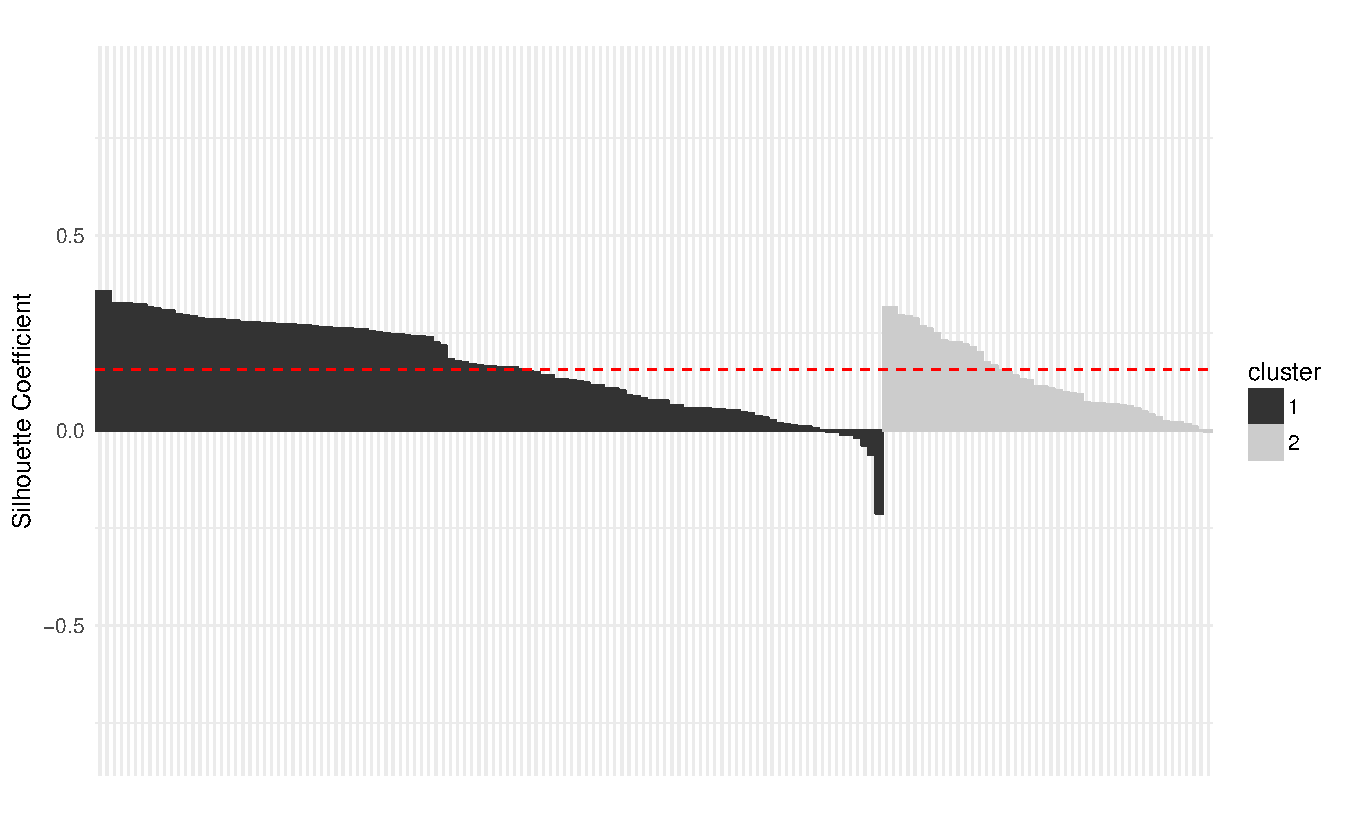
\includegraphics[width=\textwidth]{graphics/sil_ub_aligon_0.2.pdf}
        \caption{Aligon method with threshold 20\%}
    \end{subfigure}%
    ~
    \begin{subfigure}[b]{0.322\textwidth}%{0.322\textwidth}
        \centering
        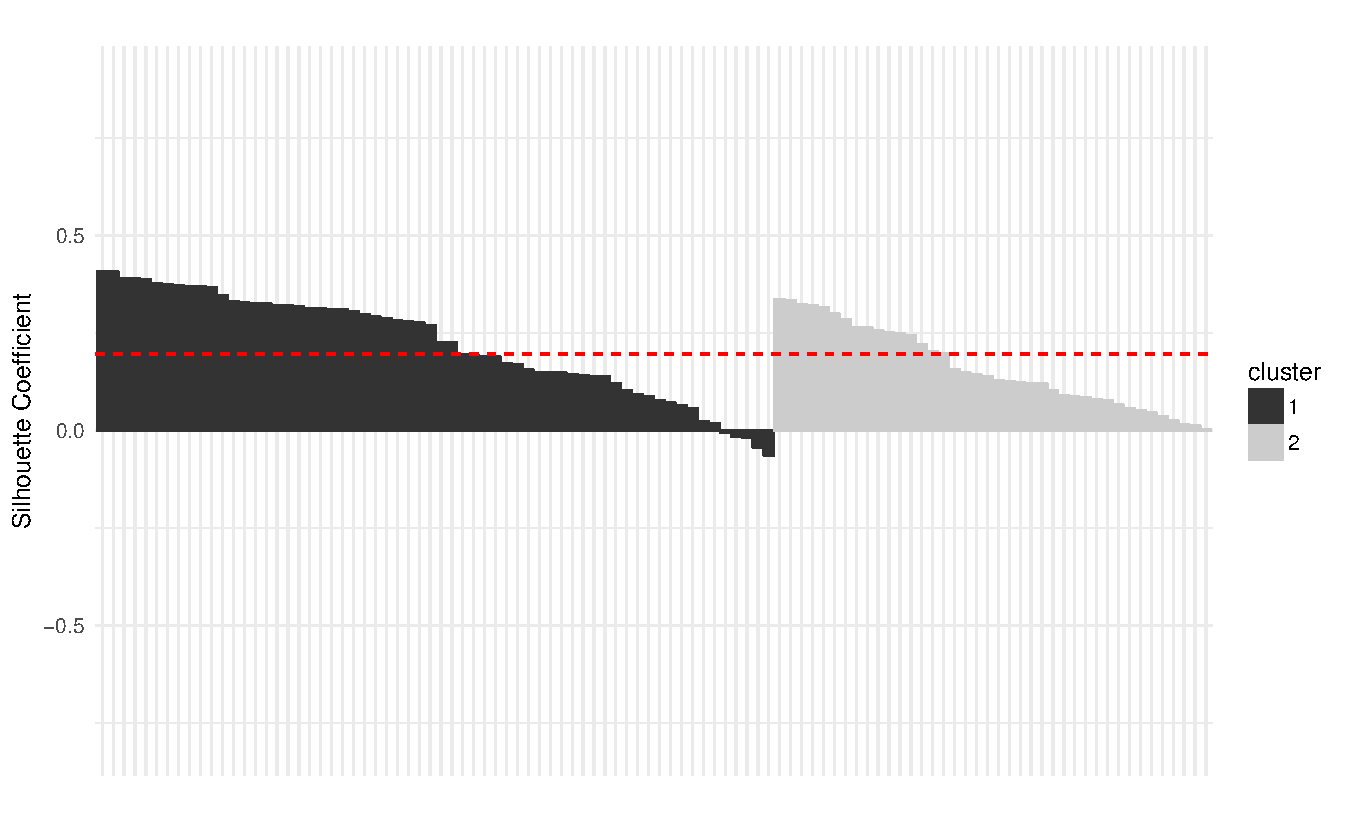
\includegraphics[width=\textwidth]{graphics/sil_ub_aligon_0.5.pdf}
        \caption{Aligon method with threshold 50\%}
    \end{subfigure}
    ~
    \begin{subfigure}[b]{0.322\textwidth}%{0.322\textwidth}
        \centering
        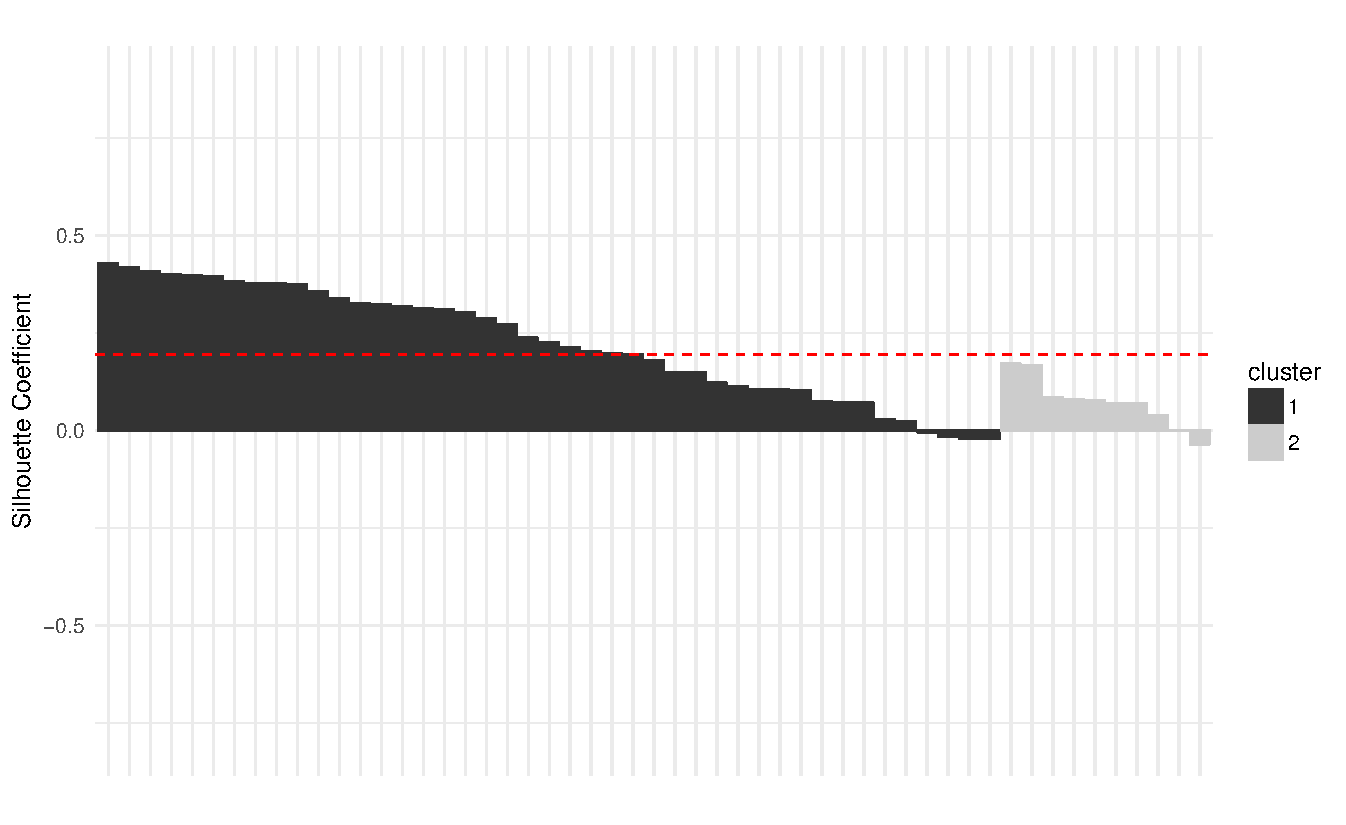
\includegraphics[width=\textwidth]{graphics/sil_ub_aligon_0.8.pdf}
        \caption{Aligon method with threshold 80\%}
    \end{subfigure}
    \\
    \begin{subfigure}[b]{0.322\textwidth}%{0.322\textwidth}
        \centering
        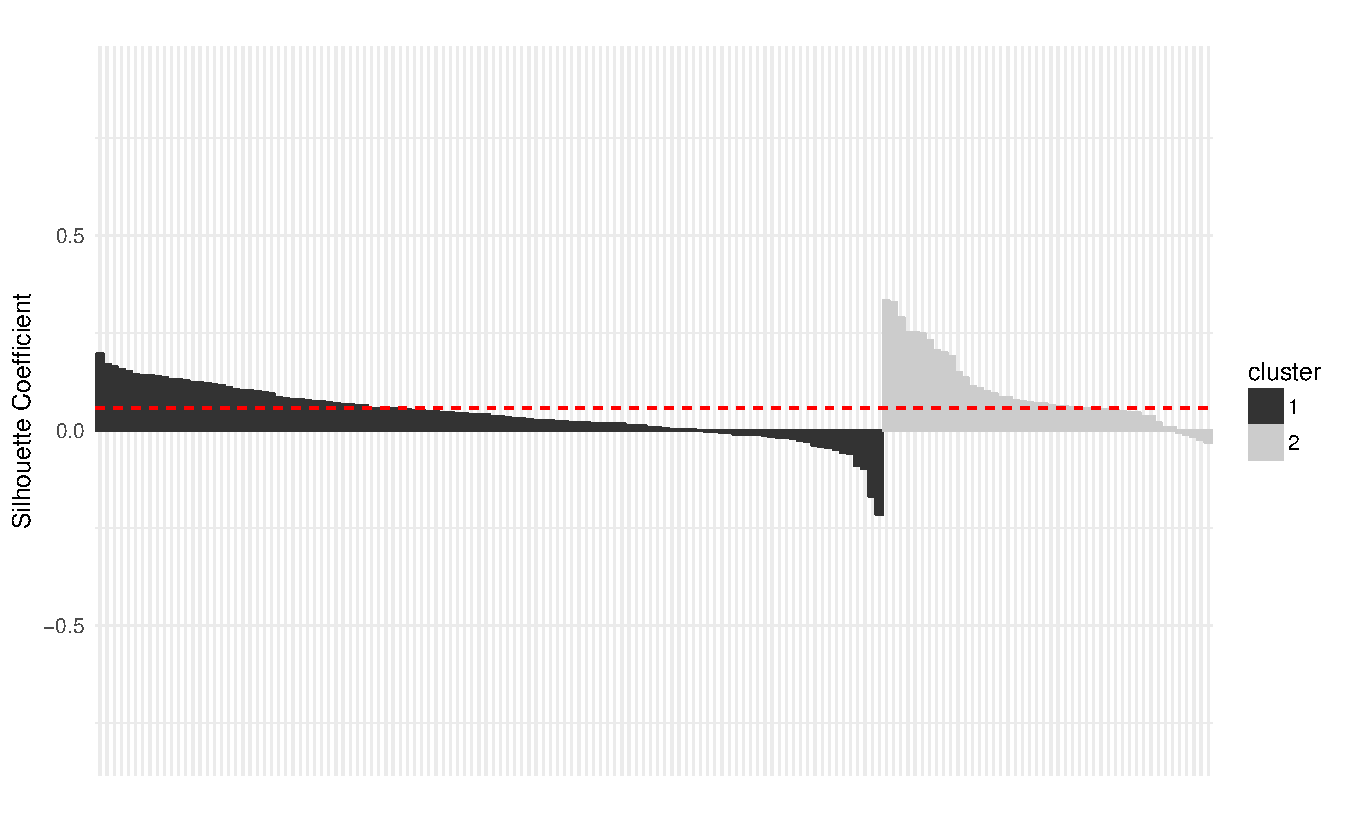
\includegraphics[width=\textwidth]{graphics/sil_ub_aouiche_0.2.pdf}
        \caption{Aouiche method with threshold 20\%}
    \end{subfigure}%
    ~
    \begin{subfigure}[b]{0.322\textwidth}%{0.322\textwidth}
        \centering
        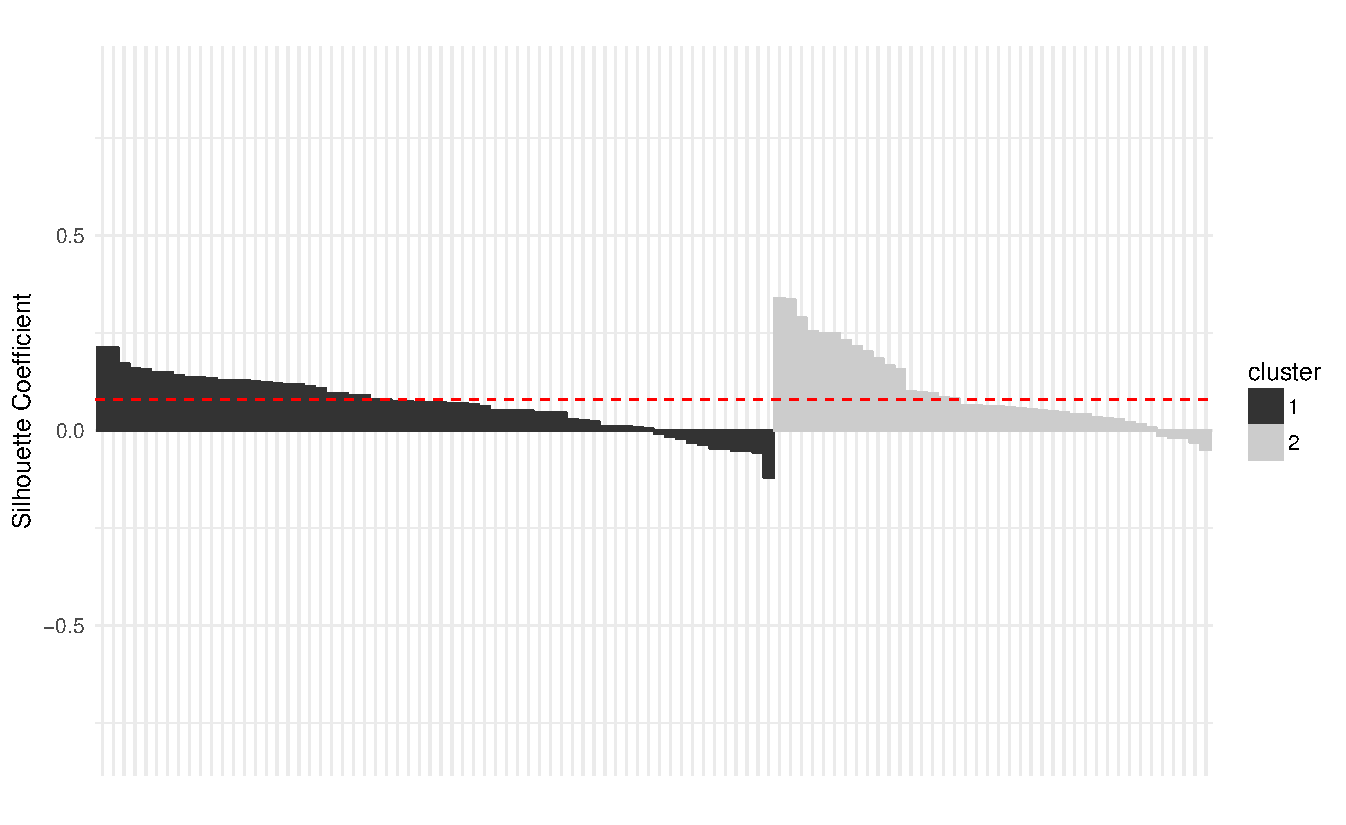
\includegraphics[width=\textwidth]{graphics/sil_ub_aouiche_0.5.pdf}
        \caption{Aouiche method with threshold 50\%}
    \end{subfigure}
    ~
    \begin{subfigure}[b]{0.322\textwidth}%{0.322\textwidth}
        \centering
        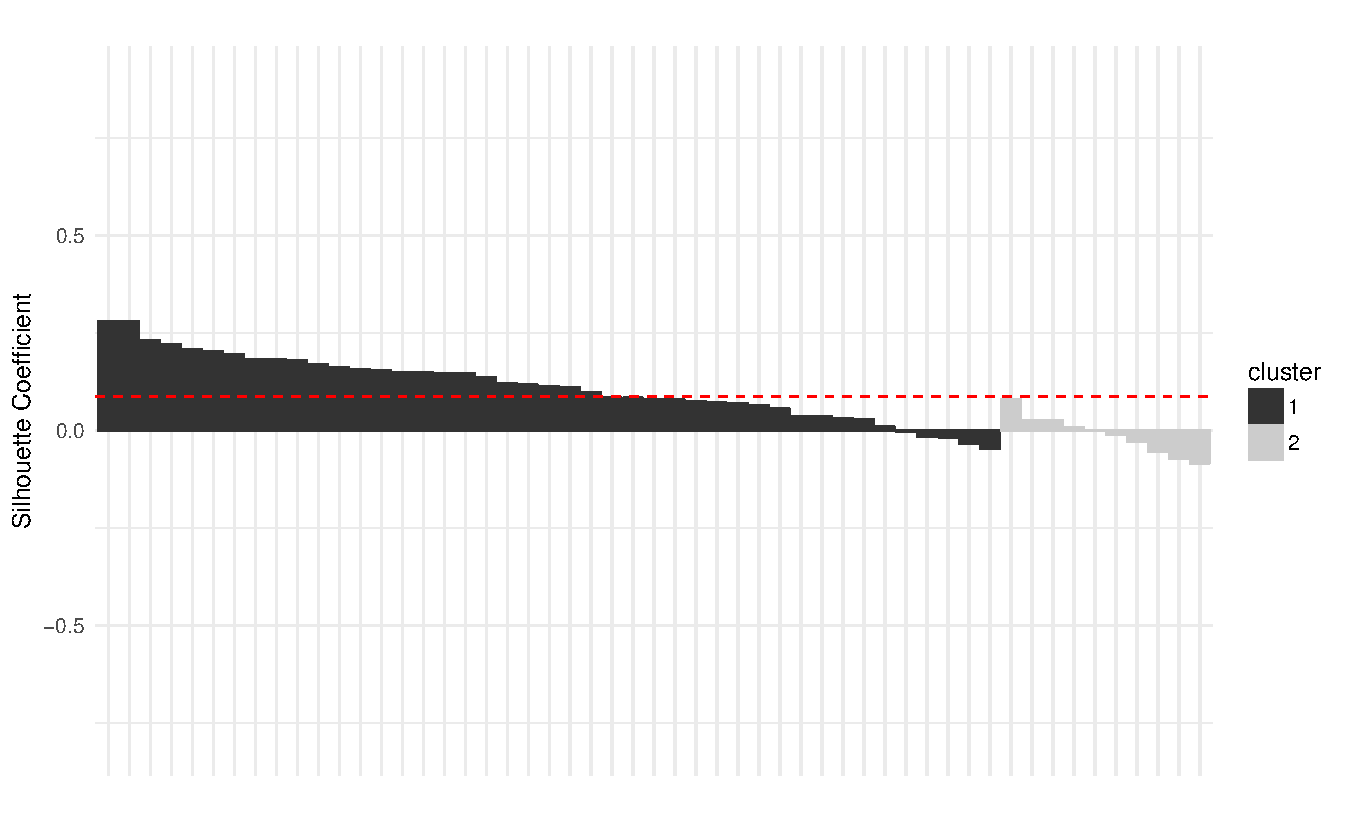
\includegraphics[width=\textwidth]{graphics/sil_ub_aouiche_0.8.pdf}
        \caption{Aouiche method with threshold 80\%}
    \end{subfigure}
    \\
    \begin{subfigure}[b]{0.322\textwidth}%{0.322\textwidth}
        \centering
        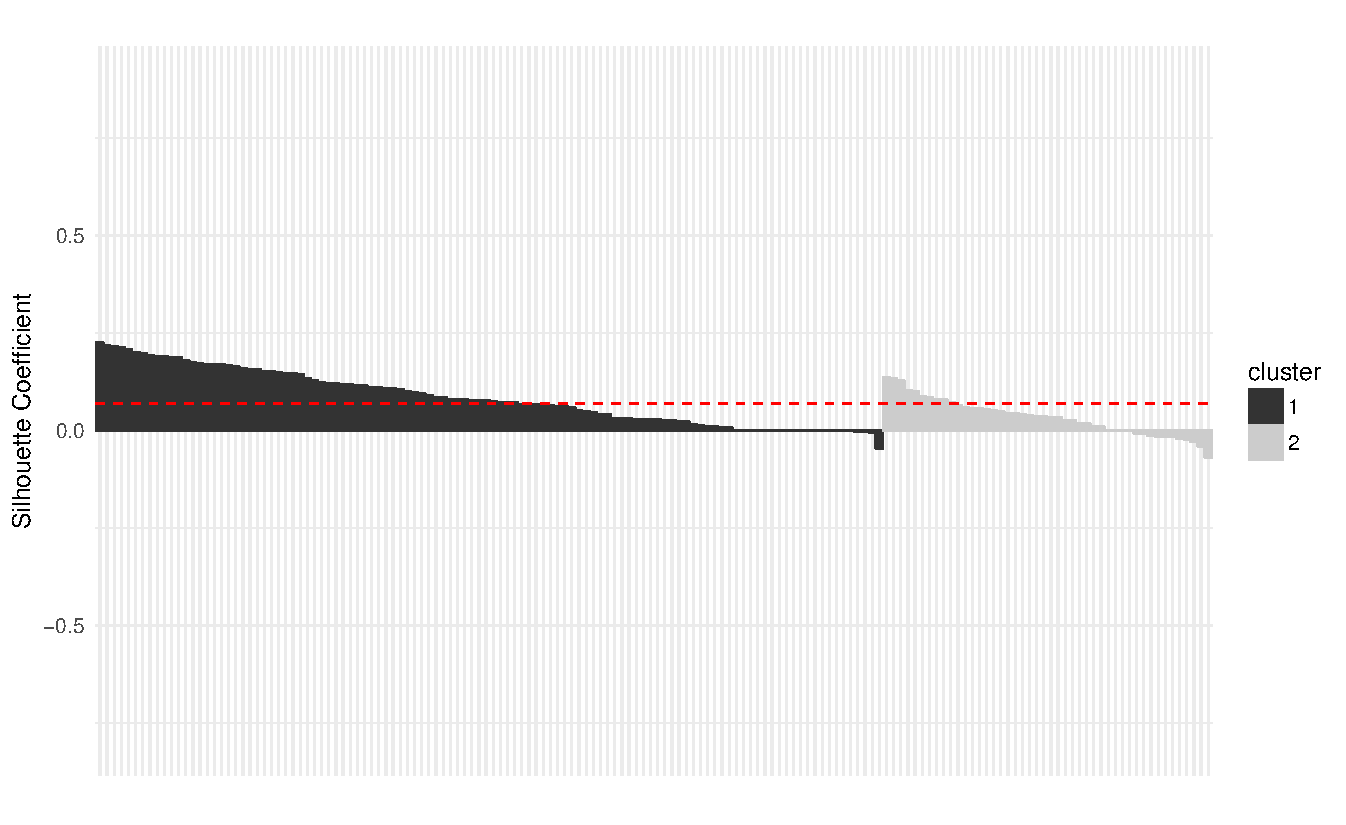
\includegraphics[width=\textwidth]{graphics/sil_ub_makiyama_0.2.pdf}
        \caption{Makiyama method with threshold 20\%}
    \end{subfigure}%
    ~
    \begin{subfigure}[b]{0.322\textwidth}%{0.322\textwidth}
        \centering
        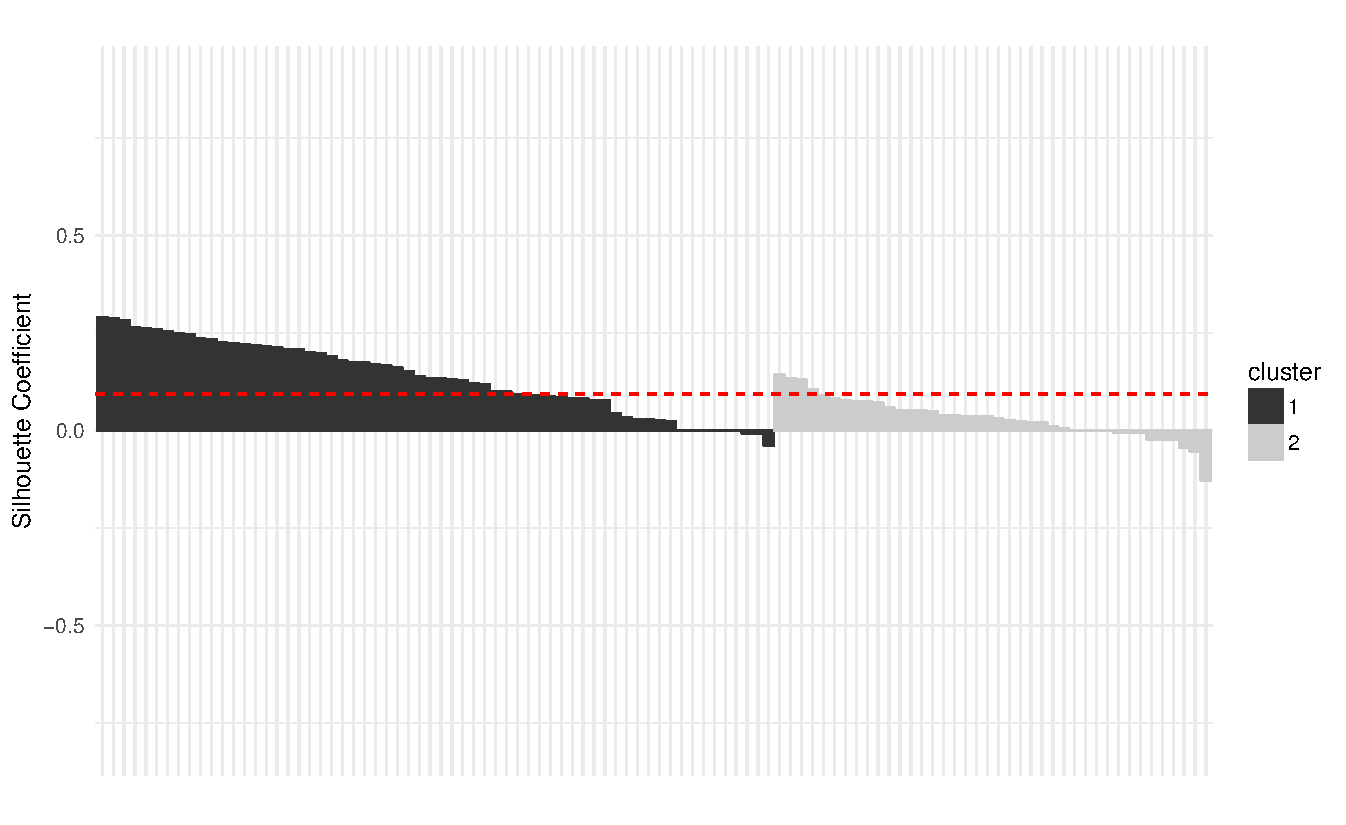
\includegraphics[width=\textwidth]{graphics/sil_ub_makiyama_0.5.pdf}
        \caption{Makiyama method with threshold 50\%}
    \end{subfigure}
    ~
    \begin{subfigure}[b]{0.322\textwidth}%{0.322\textwidth}
        \centering
        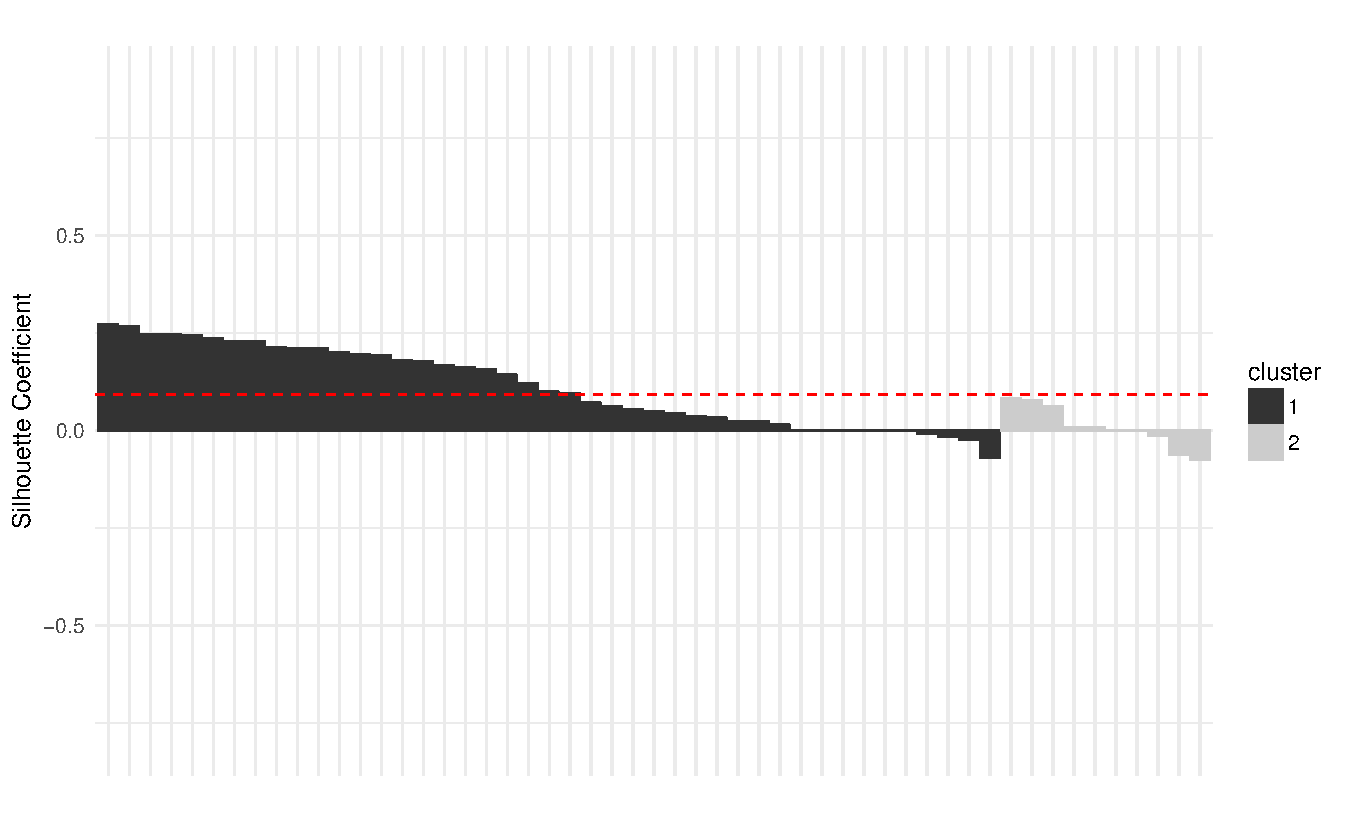
\includegraphics[width=\textwidth]{graphics/sil_ub_makiyama_0.8.pdf}
        \caption{Makiyama method with threshold 80\%}
    \end{subfigure}
    \caption{Silhouette coefficients for UB Exam Dataset when changing grading threshold in three levels - 0.2 (row 1), 0.5 (row 2), 0.8 (row 3)}
    \label{fig:sil_ub_threshold}
\end{figure*}


